\documentclass[aspectratio=169, 10pt]{beamer}

% ============================ PACKAGES ============================
\usepackage[utf8]{inputenc}
\usepackage[T1]{fontenc}
\usepackage{amsmath, amssymb, amsfonts}
\usepackage{booktabs}
\usepackage[final]{graphicx}
\usepackage{tikz}
\usetikzlibrary{shapes.geometric, arrows.meta, positioning, calc, fit, backgrounds}
\usepackage[most]{tcolorbox}

\graphicspath{{graphs/}{../graphs/}{data/results/graphs/}{./}}

% ============================ COLORS ============================
\definecolor{CreamBg}{RGB}{252, 250, 245}
\definecolor{NavyPrimary}{RGB}{20, 36, 62}
\definecolor{SlateDark}{RGB}{45, 55, 72}
\definecolor{TealAccent}{RGB}{12, 107, 133}
\definecolor{EmeraldGreen}{RGB}{15, 138, 86}
\definecolor{AmberWarm}{RGB}{194, 105, 5}
\definecolor{CoralRed}{RGB}{214, 28, 68}
\definecolor{CardBorder}{RGB}{218, 212, 200}
\definecolor{LightBlueBg}{RGB}{236, 244, 252}
\definecolor{LightTealBg}{RGB}{234, 248, 242}

% ============================ THEME ============================
\usetheme{default}
\usecolortheme{default}
\setbeamertemplate{navigation symbols}{}
\setbeamertemplate{headline}{}
\setbeamertemplate{itemize items}[circle]
\setbeamercolor{background canvas}{bg=CreamBg}
\setbeamercolor{normal text}{fg=SlateDark}
\setbeamercolor{itemize item}{fg=TealAccent}
\setbeamersize{text margin left=0.8cm, text margin right=0.8cm}
\setbeamerfont{caption}{size=\scriptsize}

% Slide number in the bottom-right corner
\setbeamertemplate{footline}{%
  \hfill{\color{SlateDark!70}\scriptsize\insertframenumber\,/\,\inserttotalframenumber}\hspace{0.8cm}\vspace{0.3cm}}

% Frame title with a thin accent line underneath
\makeatletter
\setbeamertemplate{frametitle}{
    \vspace{0.28cm}
    \begin{beamercolorbox}[wd=\paperwidth, leftskip=0.8cm, rightskip=0.8cm]{frametitle}
        {\usebeamerfont{frametitle}\color{NavyPrimary}\textbf{\insertframetitle}}
        \ifx\insertframesubtitle\@empty\else
            \\[1pt]{\color{TealAccent}\fontsize{8.5pt}{10pt}\selectfont\insertframesubtitle}
        \fi
        \\[-1pt]{\color{CardBorder}\rule{\linewidth}{0.8pt}}
    \end{beamercolorbox}
    \vspace{-0.1cm}
}
\makeatother

% ============================ CARD BOX ============================
\newtcolorbox{card}[3][]{%
  colback=white, colframe=#2, boxrule=0.9pt, arc=4pt,
  left=6pt, right=6pt, top=4pt, bottom=4pt, boxsep=1pt,
  before upper={{\bfseries\color{#2}#3\par}\vspace{3pt}},
  #1}

\newcommand{\good}[1]{{\color{EmeraldGreen}\textbf{#1}}}
\newcommand{\bad}[1]{{\color{CoralRed}\textbf{#1}}}

\begin{document}

% ====================================================================
% 1. TITLE
% ====================================================================
\begin{frame}[plain]
    \begin{tikzpicture}[remember picture, overlay]
        \fill[CreamBg] (current page.south west) rectangle (current page.north east);
        \draw[NavyPrimary, line width=3pt] ([yshift=-1.2cm]current page.north west) -- ([yshift=-1.2cm]current page.north east);
    \end{tikzpicture}

    \vspace{0.7cm}
    {\color{NavyPrimary}\LARGE \textbf{AdaLife: Adaptive SMDP Edge Caching\\[2pt] via Enhanced DDQL}}

    \vspace{0.3cm}
    {\color{TealAccent}\large \textbf{Making reinforcement learning caching work by fixing cache storage physics}}

    \vspace{1.3cm}
    \begin{columns}[onlytextwidth]
        \column{0.48\textwidth}
        \begin{card}{CardBorder}{\footnotesize\color{SlateDark} Project Candidate}
            {\color{NavyPrimary}\normalsize \textbf{CH. PP. Santosh}}
        \end{card}
        \column{0.48\textwidth}
        \begin{card}{CardBorder}{\footnotesize\color{SlateDark} Project Guide}
            {\color{NavyPrimary}\normalsize \textbf{Dr. Bheemappa Halavar}}
        \end{card}
    \end{columns}
\end{frame}

% ====================================================================
% 2. THE PROBLEM
% ====================================================================
\begin{frame}
    \frametitle{The Problem: Caching at the Network Edge}
    \framesubtitle{An edge router keeps popular files close to users so they do not wait for the far-away cloud}

    \vspace{0.2cm}
    \begin{columns}[T, onlytextwidth]
        \column{0.48\textwidth}
        \begin{card}[height=5.6cm]{CoralRed}{Why simple caching rules struggle}
            \small
            \begin{itemize}\setlength\itemsep{5pt}
                \item \textbf{Requests are random.} Users ask at random moments, not at fixed time steps.
                \item \textbf{Files are not equal.} LRU and LFU ignore file size and expiry time.
                \item \textbf{Traffic changes.} Quiet night traffic differs from busy daytime traffic, and re-training from scratch takes too long.
            \end{itemize}
        \end{card}

        \column{0.48\textwidth}
        \begin{card}[height=5.6cm, colback=LightBlueBg]{NavyPrimary}{What the base paper proposed}
            \small
            \begin{itemize}\setlength\itemsep{5pt}
                \item \textbf{Continuous-time model (SMDP).} The gap $\tau$ between requests is random, and future rewards are discounted by $\gamma^{\tau}$.
                \item \textbf{Freshness score.} A file loses value as it gets older, so stale files do not stay forever.
                \item \textbf{Transfer learning.} A policy learned in quiet hours is reused for busy hours.
            \end{itemize}
        \end{card}
    \end{columns}
\end{frame}

% ====================================================================
% 3. SYSTEM MODEL
% ====================================================================
\begin{frame}
    \frametitle{System Model: Files and Freshness}
    \framesubtitle{What the edge router stores, and how we measure how useful a file still is}

    \begin{columns}[c, onlytextwidth]
        \column{0.42\textwidth}
        \centering
        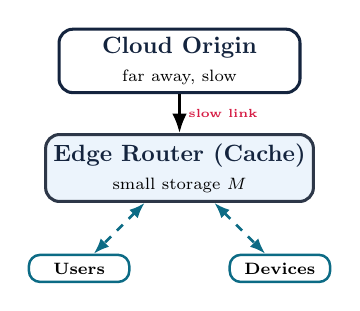
\begin{tikzpicture}[scale=0.85, transform shape]
            \node[draw=NavyPrimary, fill=white, rounded corners=5pt, line width=1.1pt, align=center, minimum width=3.6cm, minimum height=0.9cm] (cloud) at (0, 2.6) {\textbf{\color{NavyPrimary}Cloud Origin}\\ \scriptsize far away, slow};
            \node[draw=SlateDark, fill=LightBlueBg, rounded corners=5pt, line width=1.1pt, align=center, minimum width=3.6cm, minimum height=1.0cm] (router) at (0, 1.0) {\textbf{\color{NavyPrimary}Edge Router (Cache)}\\ \scriptsize small storage $M$};
            \node[draw=TealAccent, fill=white, rounded corners=4pt, line width=0.9pt, minimum width=1.5cm] (u1) at (-1.5, -0.5) {\scriptsize \textbf{Users}};
            \node[draw=TealAccent, fill=white, rounded corners=4pt, line width=0.9pt, minimum width=1.5cm] (u2) at (1.5, -0.5) {\scriptsize \textbf{Devices}};
            \draw[-{Latex[length=2.5mm]}, line width=1.1pt] (cloud) -- node[right, font=\tiny\bfseries, text=CoralRed] {slow link} (router);
            \draw[{Latex[length=2mm]}-{Latex[length=2mm]}, line width=1pt, dashed, TealAccent] (router) -- (u1);
            \draw[{Latex[length=2mm]}-{Latex[length=2mm]}, line width=1pt, dashed, TealAccent] (router) -- (u2);
        \end{tikzpicture}

        \column{0.56\textwidth}
        {\color{NavyPrimary}\textbf{Every file has four properties}}
        \begin{itemize}\small\setlength\itemsep{2pt}
            \item \textbf{Popularity $d$}: requests seen in the last $N$ requests.
            \item \textbf{Lifetime $w_l$}: how long the file stays valid.
            \item \textbf{Size $z$}: space it takes in the cache (MB).
            \item \textbf{Importance $i$}: business priority of the file.
        \end{itemize}
        \vspace{0.2cm}
        {\color{TealAccent}\textbf{Freshness}}
        \begin{itemize}\small\setlength\itemsep{2pt}
            \item Age ratio: $h^f(t) = (t - w_g^f)/w_l^f \in [0,1]$.
            \item Value drops towards $0$ as the file reaches the end of its life.
        \end{itemize}
    \end{columns}
\end{frame}

% ====================================================================
% 4. SIMULATION SETUP
% ====================================================================
\begin{frame}
    \frametitle{Simulation Setup from the Base Paper}
    \framesubtitle{Train in light traffic, then reuse the policy in heavy traffic}

    \begin{columns}[T, onlytextwidth]
        \column{0.46\textwidth}
        {\color{NavyPrimary}\textbf{Network}}
        \begin{itemize}\small\setlength\itemsep{3pt}
            \item \textbf{Files $F$:} 50 different files
            \item \textbf{Cache size $M$:} 10,000 MiB
            \item \textbf{Popularity skew:} Zipf, $\eta = 1.0$
            \item \textbf{Quiet traffic $\lambda_S$:} 0.2 requests/s
            \item \textbf{Busy traffic $\lambda_T$:} 0.3 requests/s
        \end{itemize}

        \column{0.52\textwidth}
        \vspace{0.1cm}
        \begin{table}
            \centering
            \renewcommand{\arraystretch}{1.2}
            \small
            \begin{tabular}{@{}ll@{}}
                \toprule
                \textbf{Parameter} & \textbf{Value} \\
                \midrule
                File lifetime & random, 10--30 s \\
                File size & random, 100--1000 MiB \\
                File importance & random, 0.1--0.9 \\
                Discount & $0.99^{\tau}$ \\
                Batch size & 64 transitions \\
                Replay memory & 10,000 transitions \\
                $n$-step return & 3 steps \\
                \bottomrule
            \end{tabular}
        \end{table}
    \end{columns}
\end{frame}

% ====================================================================
% 5. PAPER RESULTS
% ====================================================================
\begin{frame}
    \frametitle{Base Paper Results}
    \framesubtitle{Paper's DDQL vs.\ the CTD baseline over 5,000 requests}

    \begin{table}
        \centering
        \renewcommand{\arraystretch}{1.25}
        \resizebox{0.94\textwidth}{!}{%
        \begin{tabular}{@{}lccl@{}}
            \toprule
            \textbf{Metric} & \textbf{CTD} & \textbf{Paper DDQL} & \textbf{What it means} \\
            \midrule
            Hit rate            & 36.60\% & \textbf{62.62\%} & \good{+71\%} more requests answered locally \\
            Byte hit rate       & 34.70\% & \textbf{53.93\%} & \good{+19.2 points} more data served locally \\
            Cache misses        & 3,170   & \textbf{1,869}   & \good{$-$41\%} cloud fetches \\
            Cache evictions     & 3,152   & \textbf{250}     & \good{$-$92\%} files thrown out \\
            Total utility       & 94.17   & \textbf{190.05}  & \good{about 2$\times$} the value delivered \\
            \bottomrule
        \end{tabular}}
    \end{table}

    \vspace{0.1cm}
    \begin{columns}[T, onlytextwidth]
        \column{0.48\textwidth}
        \begin{card}{EmeraldGreen}{\scriptsize Why DDQL won}
            \scriptsize CTD removes files blindly. DDQL looks at a file's value and popularity before deciding to store it.
        \end{card}
        \column{0.48\textwidth}
        \begin{card}{CoralRed}{\scriptsize The catch}
            \scriptsize These were small synthetic runs. With heavy load and large files, the paper's policy runs into trouble (next slide).
        \end{card}
    \end{columns}
\end{frame}

% ====================================================================
% 6. FOUR GAPS
% ====================================================================
\begin{frame}
    \frametitle{Four Problems We Found in the Paper's Design}
    \framesubtitle{They showed up when we tested at larger scale}

    \vspace{0.15cm}
    \begin{columns}[T, onlytextwidth]
        \column{0.48\textwidth}
        \begin{card}[height=2.75cm]{CoralRed}{1. Evictions ignore file size}
            \footnotesize To make room for one big, rarely used file (900 MB), the cache may throw out five small, popular files (100 MB each).
        \end{card}
        \vspace{0.15cm}
        \begin{card}[height=2.75cm]{AmberWarm}{2. Empty space was punished too hard}
            \footnotesize The reward charged $100\cdot\text{Mem}$ for free space, so the agent panicked and filled the cache with useless large files.
        \end{card}

        \column{0.48\textwidth}
        \begin{card}[height=2.75cm]{SlateDark}{3. The agent could not see value per MB}
            \footnotesize The network input never told the agent whether a new file was a better use of space than the files already cached.
        \end{card}
        \vspace{0.15cm}
        \begin{card}[height=2.75cm]{TealAccent}{4. Popular files expired too early}
            \footnotesize Every file had a fixed 10--30 s timer. Even a file with 100 hits was deleted when its timer ended and had to be fetched again.
        \end{card}
    \end{columns}
\end{frame}

% ====================================================================
% 7. ADALIFE ARCHITECTURE
% ====================================================================
\begin{frame}
    \frametitle{Our Solution: AdaLife}
    \framesubtitle{We improve both the learning policy (Python) and the cache engine (Go)}

    \vspace{0.2cm}
    \centering
    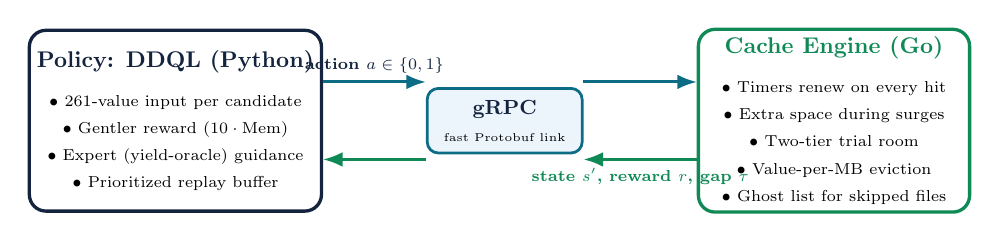
\begin{tikzpicture}[scale=0.82, transform shape]
        \node[draw=NavyPrimary, fill=white, rounded corners=6pt, line width=1.2pt, minimum width=4.2cm, minimum height=2.8cm, align=center] (py) at (0,0) {
            \textbf{\color{NavyPrimary}Policy: DDQL (Python)}\\[5pt]
            \scriptsize $\bullet$ 261-value input per candidate\\
            \scriptsize $\bullet$ Gentler reward ($10\cdot\text{Mem}$)\\
            \scriptsize $\bullet$ Expert (yield-oracle) guidance\\
            \scriptsize $\bullet$ Prioritized replay buffer};
        \node[draw=TealAccent, fill=LightBlueBg, rounded corners=4pt, line width=1pt, minimum width=2.4cm, minimum height=1.0cm, align=center] (grpc) at (5.1, 0) {\textbf{\color{NavyPrimary}\small gRPC}\\ \tiny fast Protobuf link};
        \node[draw=EmeraldGreen, fill=white, rounded corners=6pt, line width=1.2pt, minimum width=4.2cm, minimum height=2.8cm, align=center] (go) at (10.2,0) {
            \textbf{\color{EmeraldGreen}Cache Engine (Go)}\\[5pt]
            \scriptsize $\bullet$ Timers renew on every hit\\
            \scriptsize $\bullet$ Extra space during surges\\
            \scriptsize $\bullet$ Two-tier trial room\\
            \scriptsize $\bullet$ Value-per-MB eviction\\
            \scriptsize $\bullet$ Ghost list for skipped files};

        \draw[-{Latex[length=2.5mm]}, line width=1.1pt, TealAccent] ([yshift=0.6cm]py.east) -- node[above, font=\scriptsize\bfseries, text=NavyPrimary] {action $a\in\{0,1\}$} ([yshift=0.6cm]grpc.west);
        \draw[-{Latex[length=2.5mm]}, line width=1.1pt, TealAccent] ([yshift=0.6cm]grpc.east) -- ([yshift=0.6cm]go.west);
        \draw[-{Latex[length=2.5mm]}, line width=1.1pt, EmeraldGreen] ([yshift=-0.6cm]go.west) -- node[below, font=\scriptsize\bfseries, text=EmeraldGreen] {state $s'$, reward $r$, gap $\tau$} ([yshift=-0.6cm]grpc.east);
        \draw[-{Latex[length=2.5mm]}, line width=1.1pt, EmeraldGreen] ([yshift=-0.6cm]grpc.west) -- ([yshift=-0.6cm]py.east);
    \end{tikzpicture}

    \vspace{0.35cm}
    \begin{card}[width=0.94\textwidth, halign=center]{CardBorder}{\scriptsize Key idea}
        \scriptsize A better learning algorithm alone cannot fix a flawed cache. AdaLife designs the policy and the cache engine together.
    \end{card}
\end{frame}

% ====================================================================
% 8. DDQL UPGRADE
% ====================================================================
\begin{frame}
    \frametitle{Upgrade 1: A Better-Informed DDQL Agent}
    \framesubtitle{The agent now sees file size, value per MB and free space before each decision}

    \vspace{0.1cm}
    \begin{columns}[T, onlytextwidth]
        \column{0.48\textwidth}
        \begin{card}[height=5.7cm]{NavyPrimary}{10 extra features given to the agent}
            \footnotesize
            \begin{itemize}\setlength\itemsep{2pt}
                \item How often the candidate was requested recently
                \item Its exact size and its freshness-adjusted value
                \item Value density: $\rho = \text{value}/\text{size}$
                \item Lowest and average density of files in cache
                \item Gain: $\Delta\rho=\rho_{\text{cand}}-\min(\rho_{\text{cache}})$
                \item Free space, and space that must be freed
            \end{itemize}
            \textbf{Result:} the agent can weigh the trade-off directly instead of guessing.
        \end{card}

        \column{0.48\textwidth}
        \begin{card}{EmeraldGreen}{Expert (yield-oracle) guidance}
            \footnotesize The early random moves ($\epsilon\approx1$) are no longer saved as demonstrations. A simple rule based on $\Delta\rho$ and the trial-room rules supplies good examples for the supervised loss $J_E$.
        \end{card}
        \vspace{0.15cm}
        \begin{card}{TealAccent}{Fairer reward}
            \footnotesize
            $$r(t) = W^*(t) - \mathbf{10}\cdot\text{Mem}(t) - \text{Regret}_{\text{ghost}}(t)$$
            The empty-space penalty drops from 100 to 10, so the agent stops panic-caching.
        \end{card}
    \end{columns}
\end{frame}

% ====================================================================
% 9. TWO-TIER SHIELD
% ====================================================================
\begin{frame}
    \frametitle{Cache Upgrade 1: The Two-Tier Shield}
    \framesubtitle{New files first go to a ``trial room'', so one-time files cannot push out popular ones}

    \centering
    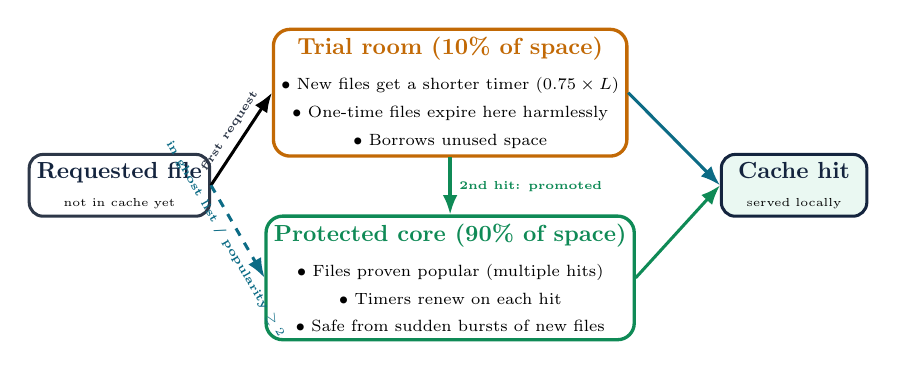
\begin{tikzpicture}[scale=0.84, transform shape]
        \node[draw=SlateDark, fill=white, rounded corners=5pt, line width=1.1pt, minimum width=2.4cm, minimum height=0.9cm, align=center] (req) at (0, 0.1) {\textbf{\color{NavyPrimary}Requested file}\\\tiny not in cache yet};
        \node[draw=AmberWarm, fill=white, rounded corners=6pt, line width=1.2pt, minimum width=4.2cm, minimum height=1.7cm, align=center] (prob) at (5.0, 1.5) {
            \textbf{\color{AmberWarm}Trial room (10\% of space)}\\[3pt]
            \scriptsize $\bullet$ New files get a shorter timer ($0.75\times L$)\\
            \scriptsize $\bullet$ One-time files expire here harmlessly\\
            \scriptsize $\bullet$ Borrows unused space};
        \node[draw=EmeraldGreen, fill=white, rounded corners=6pt, line width=1.2pt, minimum width=4.2cm, minimum height=1.7cm, align=center] (prot) at (5.0, -1.3) {
            \textbf{\color{EmeraldGreen}Protected core (90\% of space)}\\[3pt]
            \scriptsize $\bullet$ Files proven popular (multiple hits)\\
            \scriptsize $\bullet$ Timers renew on each hit\\
            \scriptsize $\bullet$ Safe from sudden bursts of new files};
        \node[draw=NavyPrimary, fill=LightTealBg, rounded corners=5pt, line width=1.1pt, minimum width=2.2cm, minimum height=0.9cm, align=center] (hit) at (10.2, 0.1) {\textbf{\color{NavyPrimary}Cache hit}\\\tiny served locally};

        \draw[-{Latex[length=2.5mm]}, line width=1.1pt] (req.east) -- node[above, sloped, font=\tiny\bfseries, text=SlateDark] {first request} (prob.west);
        \draw[-{Latex[length=2.5mm]}, line width=1.1pt, dashed, TealAccent] (req.east) -- node[below, sloped, font=\tiny\bfseries, text=TealAccent] {in ghost list / popularity $\ge 2$} (prot.west);
        \draw[-{Latex[length=2.5mm]}, line width=1.2pt, EmeraldGreen] (prob.south) -- node[right, font=\tiny\bfseries, text=EmeraldGreen] {2nd hit: promoted} (prot.north);
        \draw[-{Latex[length=2.5mm]}, line width=1.1pt, TealAccent] (prob.east) -- (hit.west);
        \draw[-{Latex[length=2.5mm]}, line width=1.1pt, EmeraldGreen] (prot.east) -- (hit.west);
    \end{tikzpicture}

    \vspace{0.3cm}
    \begin{columns}[T, onlytextwidth]
        \column{0.48\textwidth}
        \begin{card}{CardBorder}{\scriptsize\color{SlateDark} Protects against junk}
            \scriptsize A file requested only once expires in the trial room and never displaces a popular file.
        \end{card}
        \column{0.48\textwidth}
        \begin{card}{CardBorder}{\scriptsize\color{SlateDark} No wasted space}
            \scriptsize While the cache is still filling up, the trial room can use the idle space.
        \end{card}
    \end{columns}
\end{frame}

% ====================================================================
% 10. LEASES AND ELASTIC SPACE
% ====================================================================
\begin{frame}
    \frametitle{Cache Upgrade 2: Renewable Timers and Surge Space}
    \framesubtitle{Popular files stay longer, and the cache grows a little when traffic spikes}

    \vspace{0.1cm}
    \begin{columns}[T, onlytextwidth]
        \column{0.48\textwidth}
        \begin{card}[height=5.5cm]{NavyPrimary}{1. Timers that renew on every hit}
            \footnotesize Each hit extends the file's lifetime, more so for important and often-requested files:
            $$\text{boost} = 1 + 0.5\, i_f + 0.1\cdot\min(5,\text{HitCount})$$
            $$L_{\text{eff}} = \min\!\big(150\text{ s},\; L_{\text{base}}\times\text{boost}\big)$$
            \textbf{Effect:} files stay as long as users keep asking for them; unused files expire and free their space.
        \end{card}

        \column{0.48\textwidth}
        \begin{card}[height=5.5cm]{TealAccent}{2. Extra space during surges (up to +35\%)}
            \footnotesize The engine tracks the average gap between requests:
            $$\text{TauEMA} = 0.05\,\tau + 0.95\,\text{TauEMA}$$
            $$M_{\text{eff}}(t) = M\cdot(1 + 0.35\cdot\text{pressure})$$
            \textbf{Effect:} when many requests arrive at once, the cache can temporarily hold up to 35\% more, and it shrinks back safely when traffic calms down.
        \end{card}
    \end{columns}
\end{frame}

% ====================================================================
% 11. DENSITY EVICTION AND GHOST
% ====================================================================
\begin{frame}
    \frametitle{Cache Upgrade 3: Smarter Eviction and a Ghost List}
    \framesubtitle{Remove the least valuable bytes, and learn from files we wrongly skipped}

    \vspace{0.1cm}
    \begin{columns}[T, onlytextwidth]
        \column{0.48\textwidth}
        \begin{card}[height=5.5cm]{AmberWarm}{1. Evict by value per MB}
            \footnotesize The cost of fetching a file from the cloud grows with its size:
            $$C_{\text{fetch}}(f) = 0.8 + 0.4\cdot\frac{z_f}{1000}$$
            When space is needed, remove the file with the smallest
            $$\frac{y_f(t)\cdot C_{\text{fetch}}(f)}{z_f}$$
            \textbf{Effect:} no more throwing out five valuable small files for one big low-value file.
        \end{card}

        \column{0.48\textwidth}
        \begin{card}[height=5.5cm]{CoralRed}{2. Ghost list: regret for bad skips}
            \footnotesize The ghost list remembers the last 1,000 files that were skipped or evicted in the past 60 s. If one of them is requested again and misses:
            $$\text{Regret} = 5\cdot\text{UT}_{\max}\cdot i_f\cdot C_{\text{fetch}}(f)$$
            \textbf{Effect:} the regret is subtracted from the reward, so the agent quickly learns that skipping a popular file was a mistake.
        \end{card}
    \end{columns}
\end{frame}

% ====================================================================
% 12. WORKFLOW
% ====================================================================
\begin{frame}
    \frametitle{How One Request Is Handled}
    \framesubtitle{Step-by-step path of a request through AdaLife}

    \vspace{0.1cm}
    \centering
    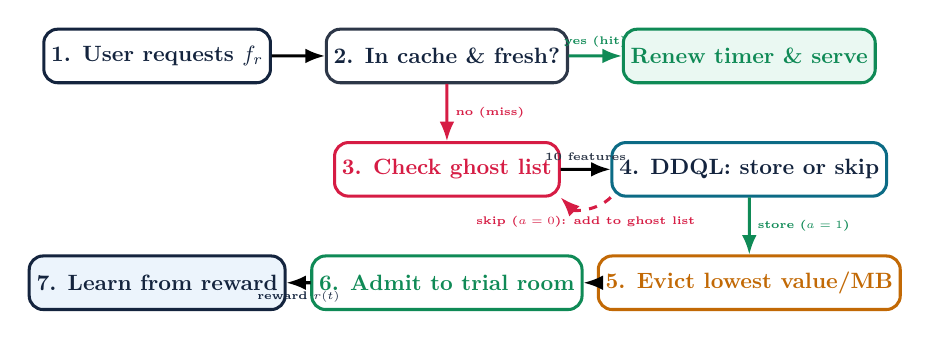
\begin{tikzpicture}[scale=0.8, transform shape]
        \node[draw=NavyPrimary, fill=white, rounded corners=5pt, line width=1.1pt, minimum width=2.8cm, minimum height=0.85cm] (req) at (0, 2.6) {\textbf{\color{NavyPrimary}1. User requests $f_r$}};
        \node[draw=SlateDark, fill=white, rounded corners=5pt, line width=1.1pt, minimum width=2.8cm, minimum height=0.85cm] (hit) at (4.6, 2.6) {\textbf{\color{NavyPrimary}2. In cache \& fresh?}};
        \node[draw=EmeraldGreen, fill=LightTealBg, rounded corners=5pt, line width=1.1pt, minimum width=3.0cm, minimum height=0.85cm] (serve) at (9.4, 2.6) {\textbf{\color{EmeraldGreen}Renew timer \& serve}};

        \node[draw=CoralRed, fill=white, rounded corners=5pt, line width=1.1pt, minimum width=2.8cm, minimum height=0.85cm] (ghost) at (4.6, 0.8) {\textbf{\color{CoralRed}3. Check ghost list}};
        \node[draw=TealAccent, fill=white, rounded corners=5pt, line width=1.1pt, minimum width=3.0cm, minimum height=0.85cm] (ddql) at (9.4, 0.8) {\textbf{\color{NavyPrimary}4. DDQL: store or skip}};

        \node[draw=AmberWarm, fill=white, rounded corners=5pt, line width=1.1pt, minimum width=3.0cm, minimum height=0.85cm] (evict) at (9.4, -1.0) {\textbf{\color{AmberWarm}5. Evict lowest value/MB}};
        \node[draw=EmeraldGreen, fill=white, rounded corners=5pt, line width=1.1pt, minimum width=2.8cm, minimum height=0.85cm] (insert) at (4.6, -1.0) {\textbf{\color{EmeraldGreen}6. Admit to trial room}};
        \node[draw=NavyPrimary, fill=LightBlueBg, rounded corners=5pt, line width=1.1pt, minimum width=2.8cm, minimum height=0.85cm] (train) at (0, -1.0) {\textbf{\color{NavyPrimary}7. Learn from reward}};

        \draw[-{Latex[length=2.5mm]}, line width=1.1pt] (req) -- (hit);
        \draw[-{Latex[length=2.5mm]}, line width=1.1pt, EmeraldGreen] (hit) -- node[above, font=\tiny\bfseries, text=EmeraldGreen] {yes (hit)} (serve);
        \draw[-{Latex[length=2.5mm]}, line width=1.1pt, CoralRed] (hit) -- node[right, font=\tiny\bfseries, text=CoralRed] {no (miss)} (ghost);
        \draw[-{Latex[length=2.5mm]}, line width=1.1pt] (ghost) -- node[above, font=\tiny\bfseries, text=SlateDark] {10 features} (ddql);
        \draw[-{Latex[length=2.5mm]}, line width=1.1pt, EmeraldGreen] (ddql) -- node[right, font=\tiny\bfseries, text=EmeraldGreen] {store ($a=1$)} (evict);
        \draw[-{Latex[length=2.5mm]}, line width=1.1pt] (evict) -- (insert);
        \draw[-{Latex[length=2.5mm]}, line width=1.1pt] (insert) -- node[below, font=\tiny\bfseries, text=NavyPrimary] {reward $r(t)$} (train);
        \draw[-{Latex[length=2.5mm]}, line width=1.1pt, dashed, CoralRed] (ddql.south west) to[out=225, in=315] node[below, font=\tiny\bfseries, text=CoralRed] {skip ($a=0$): add to ghost list} (ghost.south east);
    \end{tikzpicture}
\end{frame}

% ====================================================================
% 13. BIG BENCHMARK
% ====================================================================
\begin{frame}
    \frametitle{Large-Scale Test: 70 Million Requests}
    \framesubtitle{1,000 files, 50 GB cache, Zipf skew $\eta = 0.85$}

    \begin{table}
        \centering
        \renewcommand{\arraystretch}{1.12}
        \resizebox{0.97\textwidth}{!}{%
        \begin{tabular}{@{}lcccccc@{}}
            \toprule
            \textbf{Policy} & \textbf{Hit rate} & \textbf{Byte hit rate} & \textbf{Miss rate} & \textbf{Evicted} & \textbf{Total value} & \textbf{ns / request} \\
            \midrule
            FIFO                     & 56.04\%          & 56.31\%          & 43.96\%          & 43.96\%          & 1,810,673          & 154.5 \\
            LRU                      & 60.78\%          & 63.04\%          & 39.22\%          & 39.22\%          & 1,974,893          & \textbf{64.4} \\
            LFU                      & 68.63\%          & 69.58\%          & 31.37\%          & 31.37\%          & 2,270,792          & 116.8 \\
            Sieve (state of the art) & 69.51\%          & \textbf{71.17\%} & 30.49\%          & 30.49\%          & 2,292,812          & \textbf{61.5} \\
            CTD (paper baseline)     & 55.89\%          & 55.41\%          & 44.11\%          & 44.11\%          & 24,643,778         & 956.0 \\
            \midrule
            \textbf{Paper's DDQL}    & 66.18\%          & 46.60\%          & 33.82\%          & 22.41\%          & 22,431,459         & 26,066.5 \\
            \textbf{AdaLife (ours)}  & \textbf{78.81\%} & 61.27\%          & \textbf{21.19\%} & \textbf{14.28\%} & \textbf{37,244,712} & 20,224.0 \\
            \bottomrule
        \end{tabular}}
    \end{table}

    \vspace{0.1cm}
    \begin{columns}[T, onlytextwidth]
        \column{0.32\textwidth}
        \begin{card}{EmeraldGreen}{\scriptsize Best hit rate}
            \scriptsize AdaLife answers \textbf{78.81\%} of requests locally, ahead of every other policy.
        \end{card}
        \column{0.34\textwidth}
        \begin{card}{NavyPrimary}{\scriptsize Bandwidth recovered}
            \scriptsize Byte hit rate rises from \textbf{46.60\%} (paper's DDQL) to \textbf{61.27\%}.
        \end{card}
        \column{0.32\textwidth}
        \begin{card}{CoralRed}{\scriptsize Less churn}
            \scriptsize Only \textbf{14.28\%} of files are evicted, versus 22.41\% for the paper's DDQL.
        \end{card}
    \end{columns}
\end{frame}

% ====================================================================
% 14. FINDING 1
% ====================================================================
\begin{frame}
    \frametitle{Finding 1: Stable Learning and Good Memory Use}
    \framesubtitle{The agent learns smoothly and makes full use of the cache}

    \centering
    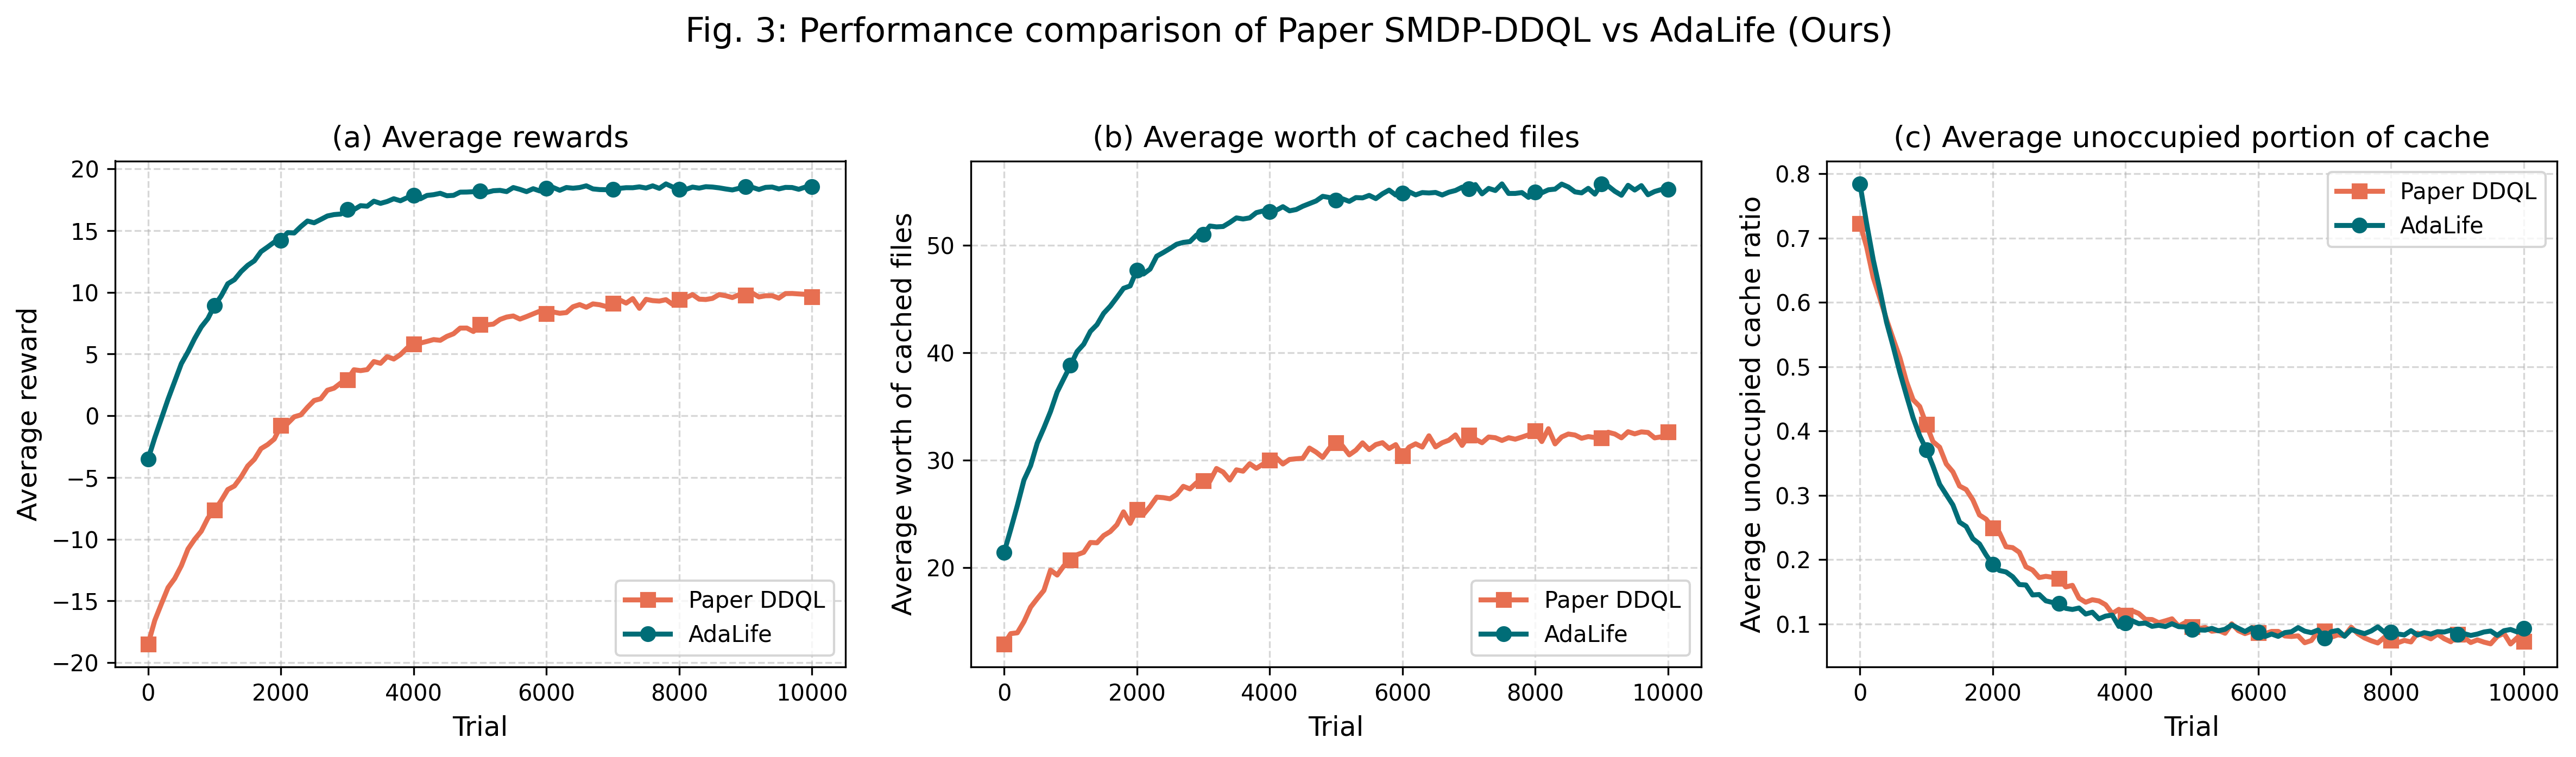
\includegraphics[width=0.90\linewidth, height=0.50\textheight, keepaspectratio]{fig3_combined_performance.png}

    \vspace{0.1cm}
    \begin{columns}[T, onlytextwidth]
        \column{0.32\textwidth}
        \textbf{\footnotesize (a) Reward}
        \begin{itemize}\scriptsize\setlength\itemsep{1pt}
            \item The policy keeps improving.
            \item Reward climbs without collapsing.
        \end{itemize}
        \column{0.34\textwidth}
        \textbf{\footnotesize (b) Stored value}
        \begin{itemize}\scriptsize\setlength\itemsep{1pt}
            \item Total value in cache stays high.
            \item Genuinely popular files are kept.
        \end{itemize}
        \column{0.32\textwidth}
        \textbf{\footnotesize (c) Empty memory}
        \begin{itemize}\scriptsize\setlength\itemsep{1pt}
            \item Unused space falls below 5\%.
            \item Storage is used effectively.
        \end{itemize}
    \end{columns}
\end{frame}

% ====================================================================
% 15. FINDING 2
% ====================================================================
\begin{frame}
    \frametitle{Finding 2: Saving Network Bandwidth}
    \framesubtitle{AdaLife repairs the drop in byte hit rate seen with the paper's DDQL}

    \begin{columns}[c, onlytextwidth]
        \column{0.52\textwidth}
        \centering
        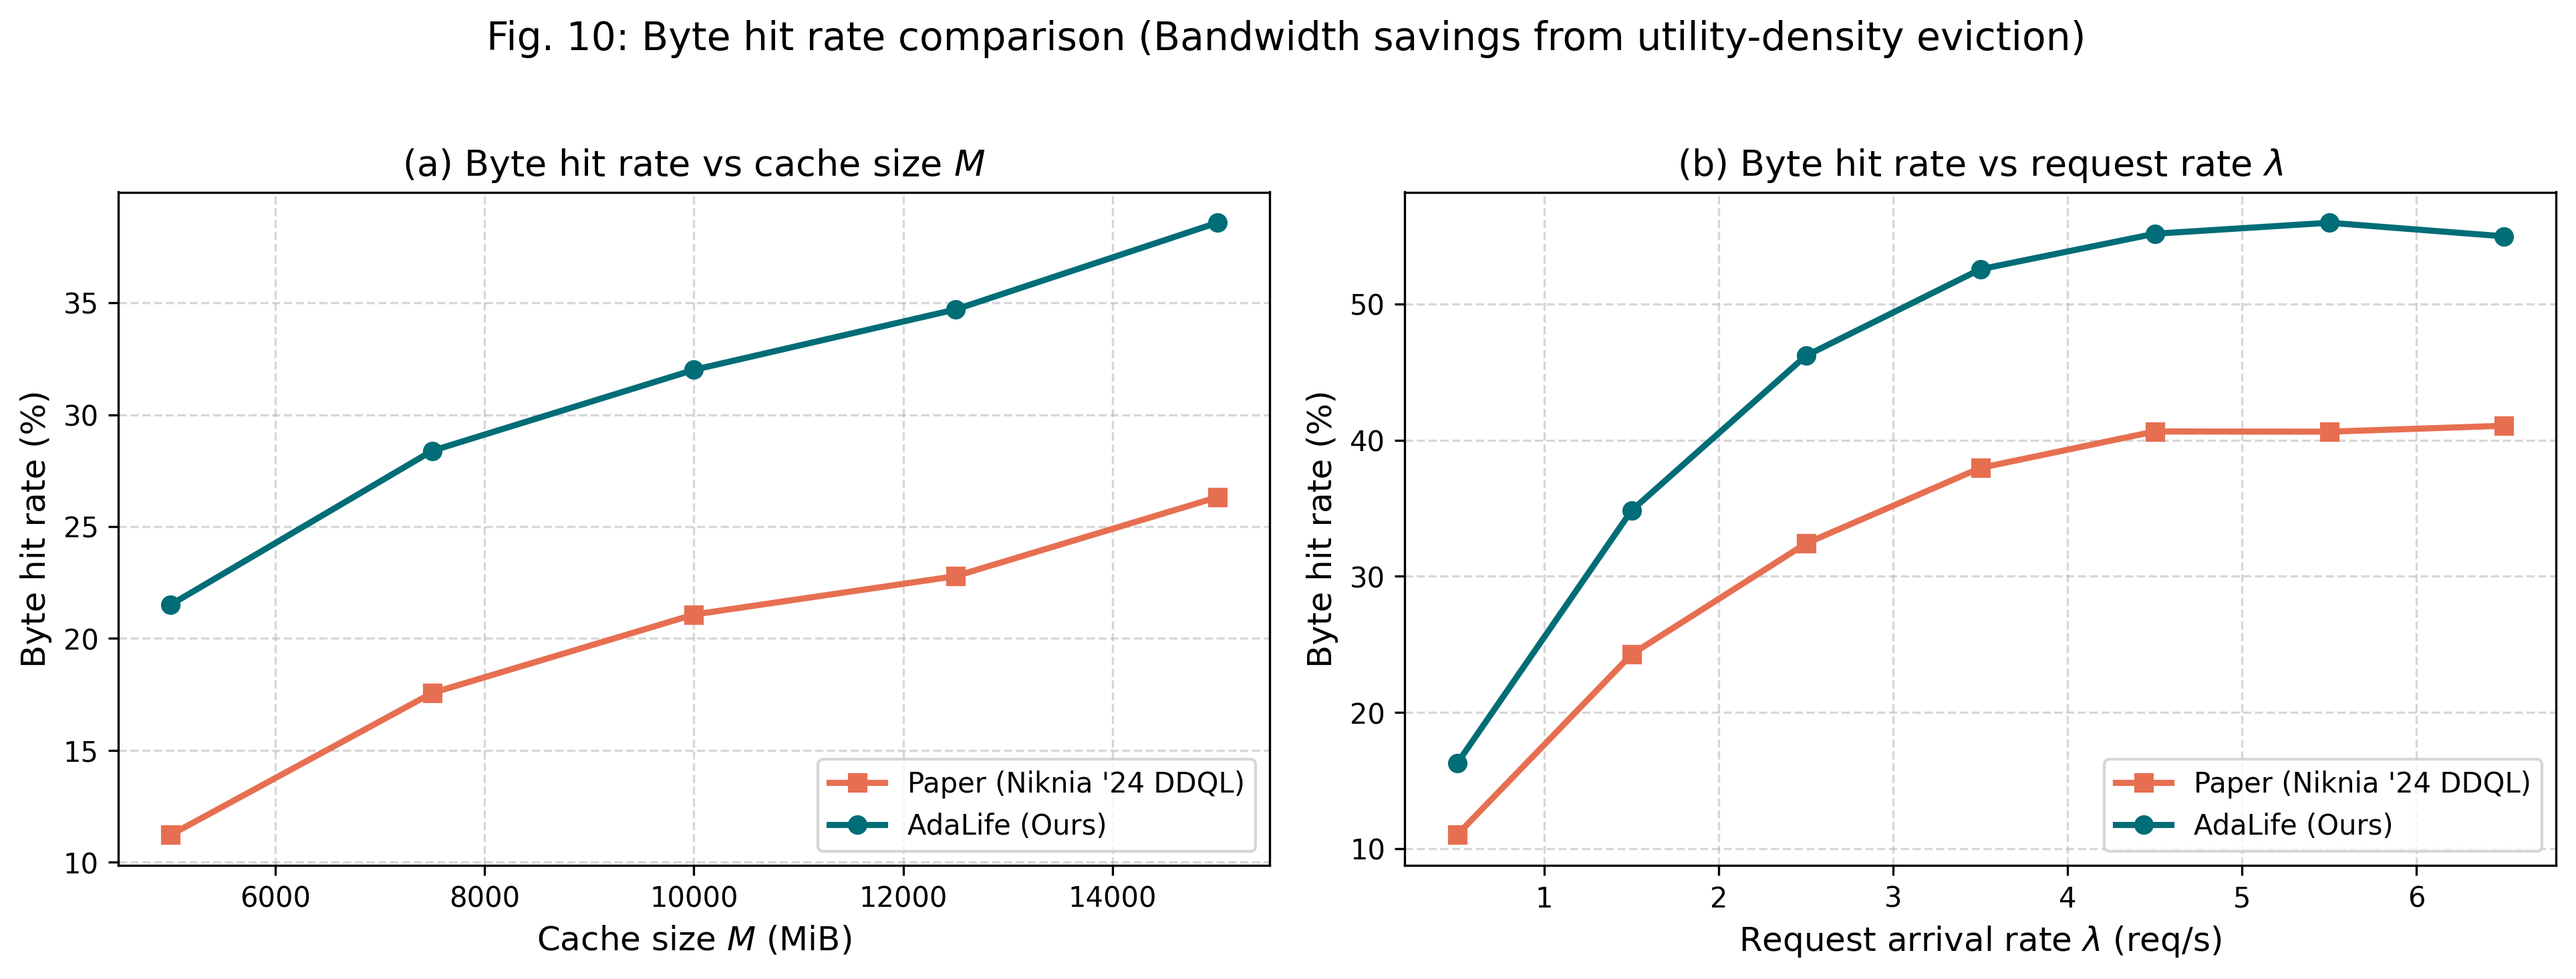
\includegraphics[width=\linewidth, height=0.72\textheight, keepaspectratio]{fig10_byte_hit_rate_comparison.png}

        \column{0.45\textwidth}
        \begin{card}{CoralRed}{The paper's bandwidth problem}
            \footnotesize The paper's hit rate was good (66\%), but its byte hit rate fell to \textbf{46.6\%}. Big files were evicted too easily and had to be downloaded again and again.
        \end{card}
        \vspace{0.2cm}
        \begin{card}{EmeraldGreen}{AdaLife: 61.27\%}
            \footnotesize Value-per-MB eviction keeps big files when they are worth it. Data fetched from the cloud drops by about 27\%.
        \end{card}
    \end{columns}
\end{frame}

% ====================================================================
% 16. FINDING 3
% ====================================================================
\begin{frame}
    \frametitle{Finding 3: Less Cache Thrashing}
    \framesubtitle{The trial room stops popular files from being pushed out}

    \begin{columns}[c, onlytextwidth]
        \column{0.52\textwidth}
        \centering
        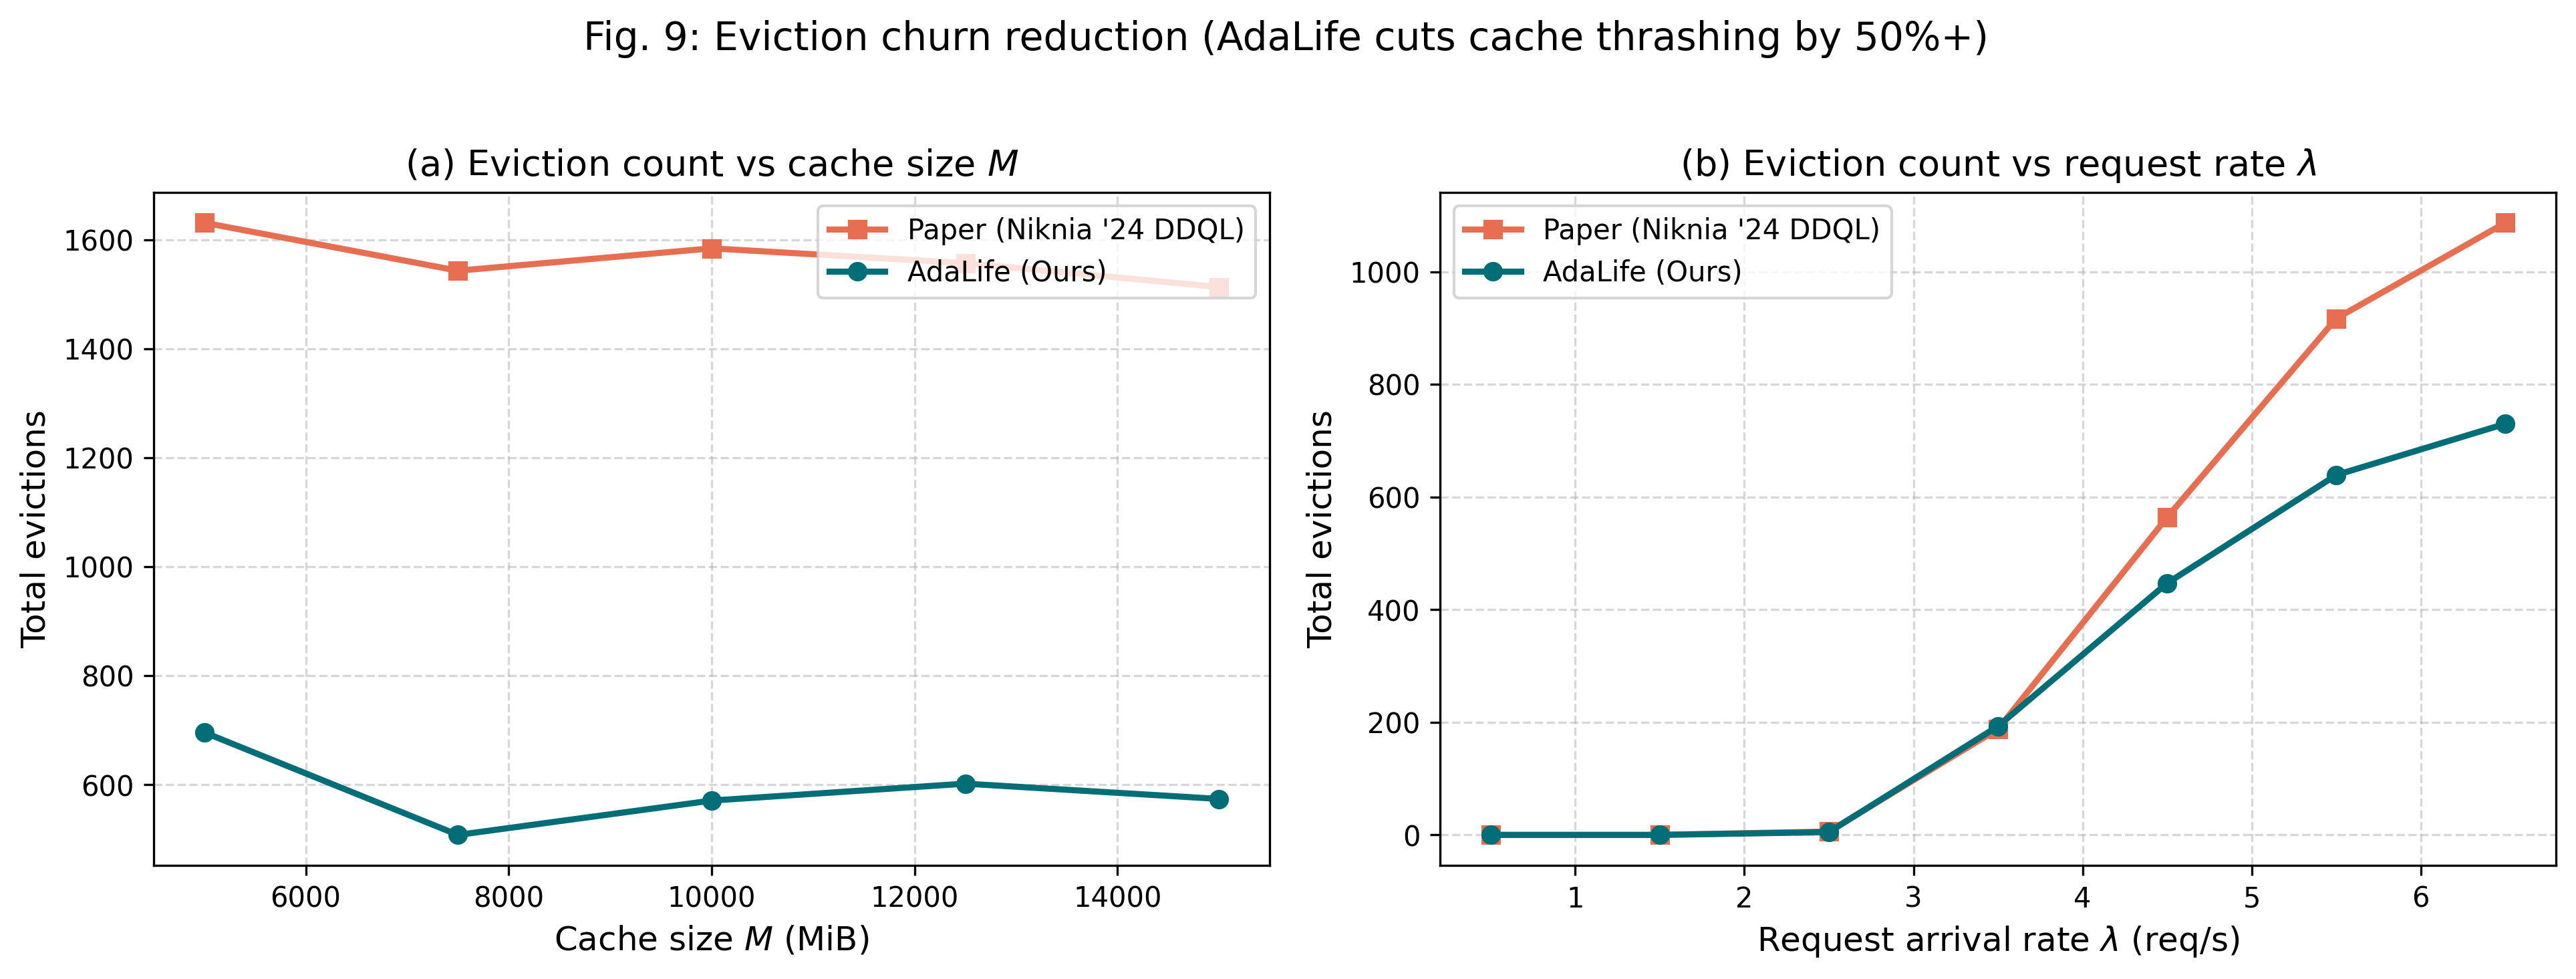
\includegraphics[width=\linewidth, height=0.72\textheight, keepaspectratio]{fig9_eviction_churn_comparison.png}

        \column{0.45\textwidth}
        \begin{card}{CoralRed}{Classic policies thrash}
            \footnotesize FIFO, LRU, LFU and Sieve evict \textbf{30--44\% of files}. A burst of new files pushes out popular ones before they can serve more hits.
        \end{card}
        \vspace{0.2cm}
        \begin{card}{EmeraldGreen}{AdaLife: only 14.28\%}
            \footnotesize New files wait in the 10\% trial room, so the main storage stays protected. Fewer deletions also means less disk wear on the router.
        \end{card}
    \end{columns}
\end{frame}

% ====================================================================
% 17. FINDING 4 (REPLACED: DIRECT COMPARISON ACROSS SYSTEM CONDITIONS)
% ====================================================================
\begin{frame}
    \frametitle{Finding 4: Higher Hit Counts Across All Network Conditions}
    \framesubtitle{AdaLife vs.\ Paper's DDQL across popularity skew, request rate, and cache size}

    \centering
    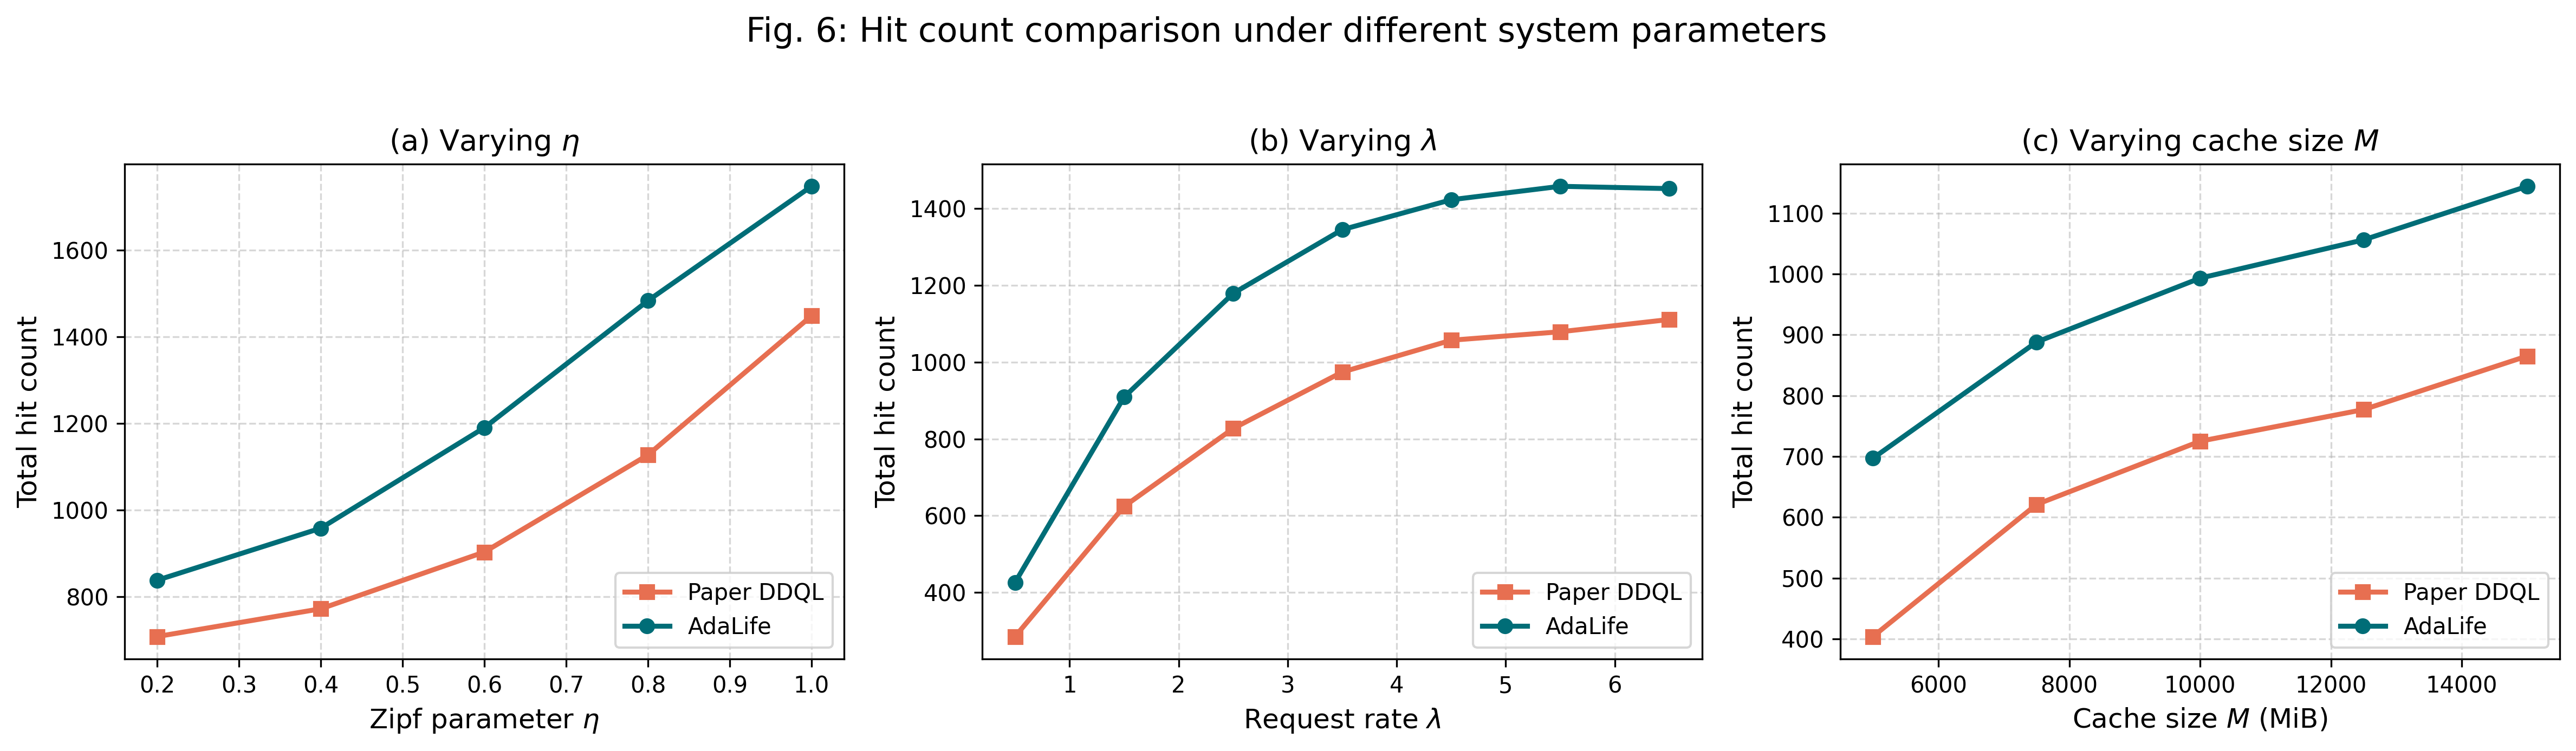
\includegraphics[width=0.92\linewidth, height=0.48\textheight, keepaspectratio]{fig6_combined_hit_counts.png}

    \vspace{0.1cm}
    \begin{columns}[T, onlytextwidth]
        \column{0.32\textwidth}
        \textbf{\footnotesize (a) Popularity Skew ($\eta$)}
        \begin{itemize}\scriptsize\setlength\itemsep{1pt}
            \item AdaLife stays well above Paper DDQL for every skew value.
            \item Leases preserve the most popular files.
        \end{itemize}
        \column{0.34\textwidth}
        \textbf{\footnotesize (b) Request Rate ($\lambda$)}
        \begin{itemize}\scriptsize\setlength\itemsep{1pt}
            \item Evaluated from light to heavy traffic ($0.5$--$6.5$ req/s).
            \item AdaLife widens its lead as traffic grows.
        \end{itemize}
        \column{0.32\textwidth}
        \textbf{\footnotesize (c) Cache Capacity ($M$)}
        \begin{itemize}\scriptsize\setlength\itemsep{1pt}
            \item Tested across tight (5 GB) to large (15 GB) caches.
            \item Consistently delivers more hits at all sizes.
        \end{itemize}
    \end{columns}
\end{frame}

% ====================================================================
% 18. SUMMARY
% ====================================================================
\begin{frame}
    \frametitle{Summary}
    \framesubtitle{What AdaLife achieves}

    \vspace{0.15cm}
    \begin{columns}[T, onlytextwidth]
        \column{0.31\textwidth}
        \begin{card}[height=4.4cm]{NavyPrimary}{1. A better-informed agent}
            \footnotesize
            \begin{itemize}\setlength\itemsep{3pt}
                \item 10 extra features show value per MB.
                \item Gentler reward stops panic hoarding.
                \item Yield-oracle guides target training.
            \end{itemize}
        \end{card}
        \column{0.31\textwidth}
        \begin{card}[height=4.4cm]{EmeraldGreen}{2. A smarter cache}
            \footnotesize
            \begin{itemize}\setlength\itemsep{3pt}
                \item Timers renew on every hit.
                \item Trial room blocks one-time files.
                \item Ghost list punishes bad skips.
                \item Value-per-MB eviction.
            \end{itemize}
        \end{card}
        \column{0.31\textwidth}
        \begin{card}[height=4.4cm]{TealAccent}{3. Proven at 70M requests}
            \footnotesize
            \begin{itemize}\setlength\itemsep{3pt}
                \item \textbf{78.8\%} hit rate, the best of all policies.
                \item \textbf{61.3\%} byte hit rate (+14.7 points over the paper's DDQL).
                \item \textbf{37.2M} total value (about 1.66$\times$ the paper's DDQL).
            \end{itemize}
        \end{card}
    \end{columns}

    \vspace{0.3cm}
    \begin{card}[width=0.96\textwidth, halign=center]{CardBorder}{\scriptsize Final takeaway}
        \scriptsize A learned policy only works as well as the cache underneath it. By fixing the cache and the policy together, AdaLife turns good decisions into real hit-rate gains.
    \end{card}
\end{frame}

% ====================================================================
% 19. REFERENCES
% ====================================================================
\begin{frame}
    \frametitle{References}
    \framesubtitle{Foundational Literature}

    \vspace{0.3cm}
    \begin{card}{NavyPrimary}{Key Literature}
        \small
        \begin{enumerate}\setlength\itemsep{12pt}
            \item[{[1]}] F.~Niknia, P.~Wang, Z.~Wang, A.~Agarwal, and A.~S.~Rezaei, ``Edge Caching Based on Deep Reinforcement Learning and Transfer Learning,'' \textit{arXiv preprint arXiv:2402.14576v2 [cs.NI]}, Mar.~2024.
            \item[{[2]}] H.~Zhu, Y.~Cao, X.~Wei, W.~Wang, T.~Jiang, and S.~Jin, ``Caching Transient Data for Internet of Things: A Deep Reinforcement Learning Approach,'' \textit{IEEE Internet of Things Journal}, vol.~6, no.~2, pp.~2074--2083, 2018.
        \end{enumerate}
    \end{card}
\end{frame}

% ====================================================================
% 20. THANK YOU
% ====================================================================
\begin{frame}[plain]
    \begin{tikzpicture}[remember picture, overlay]
        \fill[CreamBg] (current page.south west) rectangle (current page.north east);
        \draw[NavyPrimary, line width=3pt] ([yshift=-1.2cm]current page.north west) -- ([yshift=-1.2cm]current page.north east);
    \end{tikzpicture}

    \centering
    \vspace{2.8cm}
    {\fontsize{34pt}{40pt}\selectfont \color{NavyPrimary}\textbf{THANK YOU}}

    \vspace{0.6cm}
    
\begin{tikzpicture}
        \draw[TealAccent, line width=1.5pt] (0,0) -- (4.5,0);
    \end{tikzpicture}

    \vspace{0.5cm}
    {\color{SlateDark}\large Questions?}
\end{frame}

\end{document}
